\documentclass[main.tex]{subfiles}

\begin{document}

\section{Description of the simulation}

\subsection{Poisson Process}

The Poisson process is a stochastic process where events happen randomly but at a constant rate $\lambda$. 
An example of this is the number of photons that are measured in a detector in a given time, or the number of radioactive decay. 
It is also useful as a model of logistic problems such as the number of incoming calls to a call center. 

\begin{itemize}
    \item Make a simulation of a Poisson process. Assume that the rate at which the events occur is 3 events per second. Simulate 100 seconds and make a plot of a single realization of this process.
    \item Run the simulation many times (more than 10,000) and make a histogram of  after 0, 25, 50, 75 and 100 seconds. Plot all the histograms on the same axis.
    \item Plot the average of all the runs for every instant $\expval{N(t)}$ and the variance $\sigma^2(N(t))$. What is the average number of events that occurred after 100 sec? Is this what you would expect?
\end{itemize}

\subsection{Birth and Death Process}

We can generalize the Poisson process to one in which something appears and disappears. 
This could be, for example, a population where individuals live and die at constant rates. 
For this, we will define a state variable $n(t)$, which represents the number of people in the population. 
When a person is born we add 1 to the variable n and when a person dies we subtract 1. 

\begin{itemize}
    \item Adapt your algorithm to simulate a Birth and Death Process. Assume that the birth rate is $\beta=3$ births per second and the death rate $\gamma=1$ is deaths per second.
    \item As before, run the simulation many times, plot the histograms for 0, 25, 50, 75, and 100 seconds, and the mean and variance.
\end{itemize}

\section{Poisson Process}

An intuitive example that can be described as a Poisson process is the calls receive in a call center, where is expected to receive $m$ calls per hour, but we ignore the exact minute in which the calls are made.
It is commonly represented the probability of receive a call receive per minute with $\lambda$ and refers to it as a rate.
Therefore, considering that is a constant rate of events, it is expected a constant increment in the quantity of calls by every hour that has passed.

A way to describe mathematically this process is to define a random variable $N$ that can be \num{0} or \num{1}, representing if there was a call or not, with the probability of getting \num{1} of $\lambda t$ and a probability of getting \num{0} of $1-\lambda t$,
\begin{gather}
    N = \left\{
        \begin{array}{ll}
            0, & P(0) = 1-\lambda t \\
            1, & P(1) = \lambda t
        \end{array}
    \right.
    .\label{eqn5:poissonProcess}
\end{gather}
The reason of including the parameter $t$ in the probability can be explained as follows, knowing that $\lambda$ is a rate of the probability of the event per temporal unit and we want to know the probability of the event, we just multiply it by a fraction of the temporal unit $t$ to get the probability of the event in a instant.

It is important to note that the variable $N$ is occurs at an instant in time, while the definition of the probability is introduce by an average of events in a time span.
Taking that into account, a single realization of this process it involves $n$ events in a temporal range.

\subsection{Simulations}

Considering that the rate of events is $\lambda = 3$, the instant $t$ is set to $\SI{1d-2}{\second}$ the probability of getting a success is $P(1) = 0.03$.
Considering that we are respecting to have 3 successes in a second, the number of successes in 100 seconds should be near 300.
In the figure \ref{fig:poissonProcess} it is shown the number of successes receive in a time span of 100 seconds and in fact, the number of successes at 100 of seconds is near 300.

\begin{figure}[ht!]
    \centering
    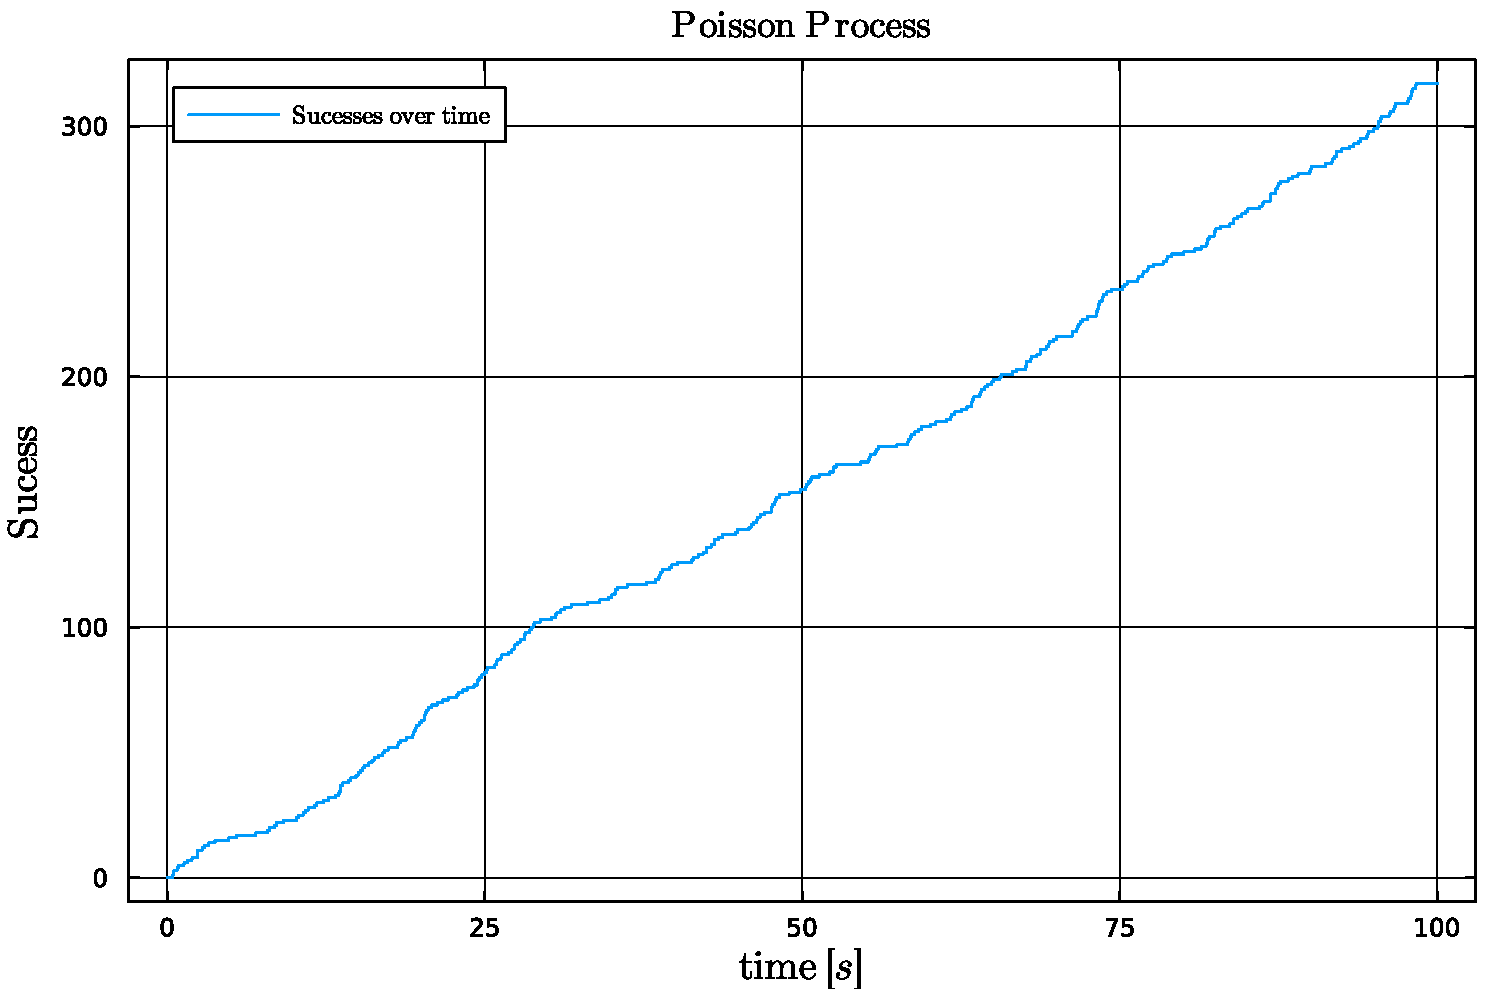
\includegraphics[width=0.8\textwidth]{imgs/hw5/poissonProcess.pdf}
    \caption{Number of success in a Poisson process with $\lambda=3$ in a time span of 100 seconds.}
    \label{fig:poissonProcess}
\end{figure}

On the other hand, in the figure \ref{fig:poissonProcessHisto} it is shown a histogram of the number of successes after 0, 25, 50, 75 and 100 seconds from a data set of \num{20000} realizations.
In which a it can be appreciated a shift in the mean of the number of successes at a increasing time, also it can be observed that at a bigger time, the distribution of the number of successes spreads out.

\begin{figure}[ht!]
    \centering
    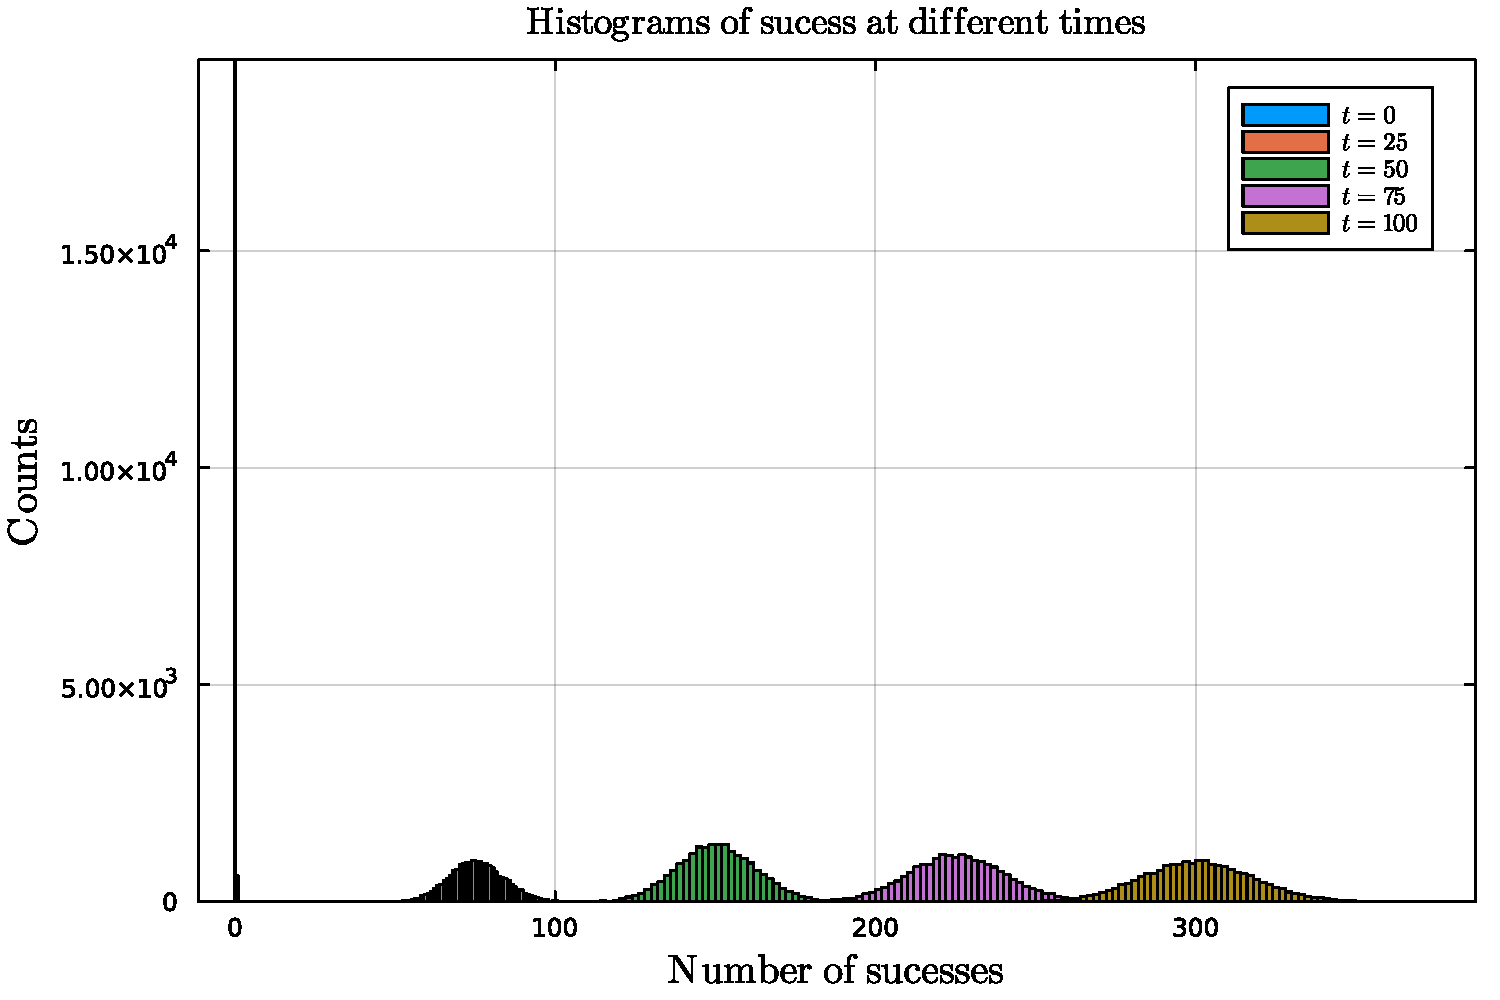
\includegraphics[width=0.8\textwidth]{imgs/hw5/poissonProcessHistograms.pdf}
    \caption{
    Evolution of the number of success of a data set of \num{20000} realizations at different instants.
    }
    \label{fig:poissonProcessHisto}
\end{figure}

Finally, in the figure \ref{fig:poissonProcessMeanVar} the average and the variance of successes in the time span are shown.
The initial hypothesis of expecting a constant rate of success per second due to the interpretation of $\lambda$, it can be reassure by the graph of the mean over time, which it is a straight line with a slope of $\lambda$.
On the other hand, the variance has an equal behavior to the mean and when we consider that the variance can be use as a measure of how much the data is "spread", it indicates that the distribution of the number of success is going to spread out at a constant rate thru time, as shown in figure \ref{fig:poissonProcessHisto}.

\begin{figure}[ht!]
    \centering
    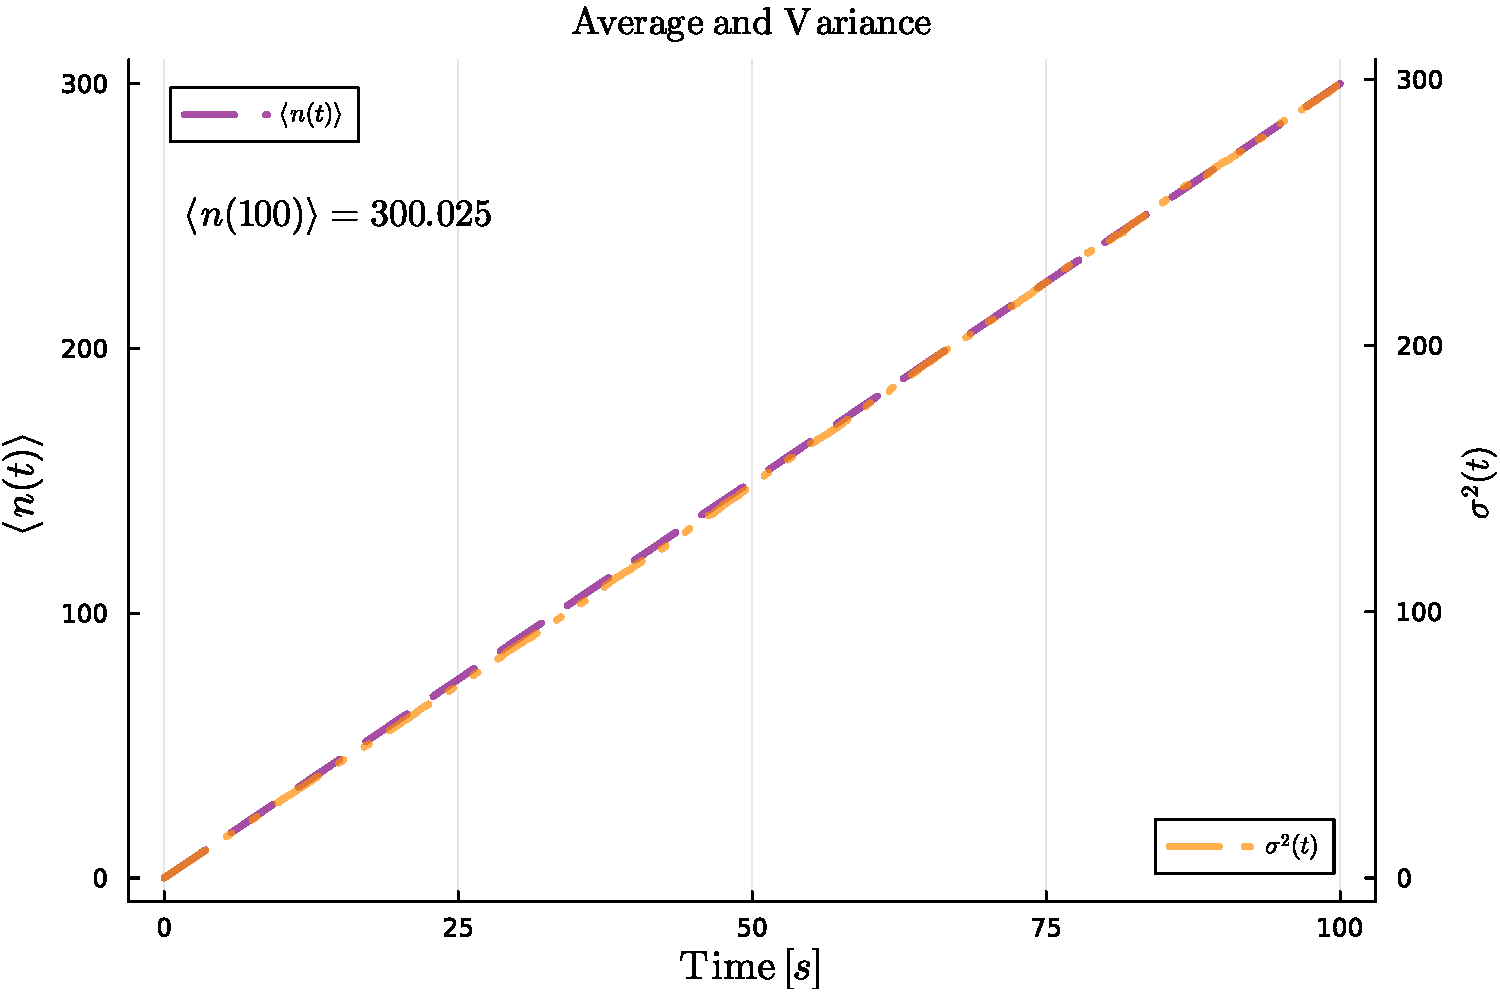
\includegraphics[width=0.8\textwidth]{imgs/hw5/poissonProcessAvergeVariance.pdf}
    \caption{Mean and the variance of a data set of \num{20000} realizations of a Poisson process in a time span of 100 seconds.}
    \label{fig:poissonProcessMeanVar}
\end{figure}

\section{Birth and Death Process}

Now, modifying the equation \eqref{eqn5:poissonProcess} to adapt it to simulate a birth and death process with birth rate of $\beta$ and a death process of $\gamma$, 
\begin{gather}
    N = \left\{
        \begin{array}{ll}
            -1, & P(-1) = \gamma t \\
            0, & P(0) = 1-\qty(\beta+\gamma)t \\
            1, & P(1) = \beta t
        \end{array}
    \right.
    .\label{eqn5:birthdeath}
\end{gather}
The reason that the probability that nothing happens is the sum of the birth with the death probabilities and not the difference it is because it is need a complementary state that helps to ensure that the sum of probabilities is equal to one. % Try to improve this sentence.

\subsection{Simulations}

Taking into account that the rates are given by state per second, the variable $t$ is set to $\SI{1d-2}{\second}$, causing the following probabilities for each event,
\begin{gather*}
    N = \left\{
        \begin{array}{ll}
            -1, & P(-1) = 0.01 \\
            0, & P(0) = 0.96 \\
            1, & P(1) = 0.03
        \end{array}
    \right.
    .%\label{eqn5:birthdeath}
\end{gather*}

In figure \ref{fig:bdProcessHisto} is shown a set of histogram of the population after 0, 25, 50, 75 and 100 seconds using a date set of \num{20000} realizations and the average and variance of the population in the time span is displayed in figure \ref{fig:bdProcessMeanVar} .

\begin{figure}[ht!]
    \centering
    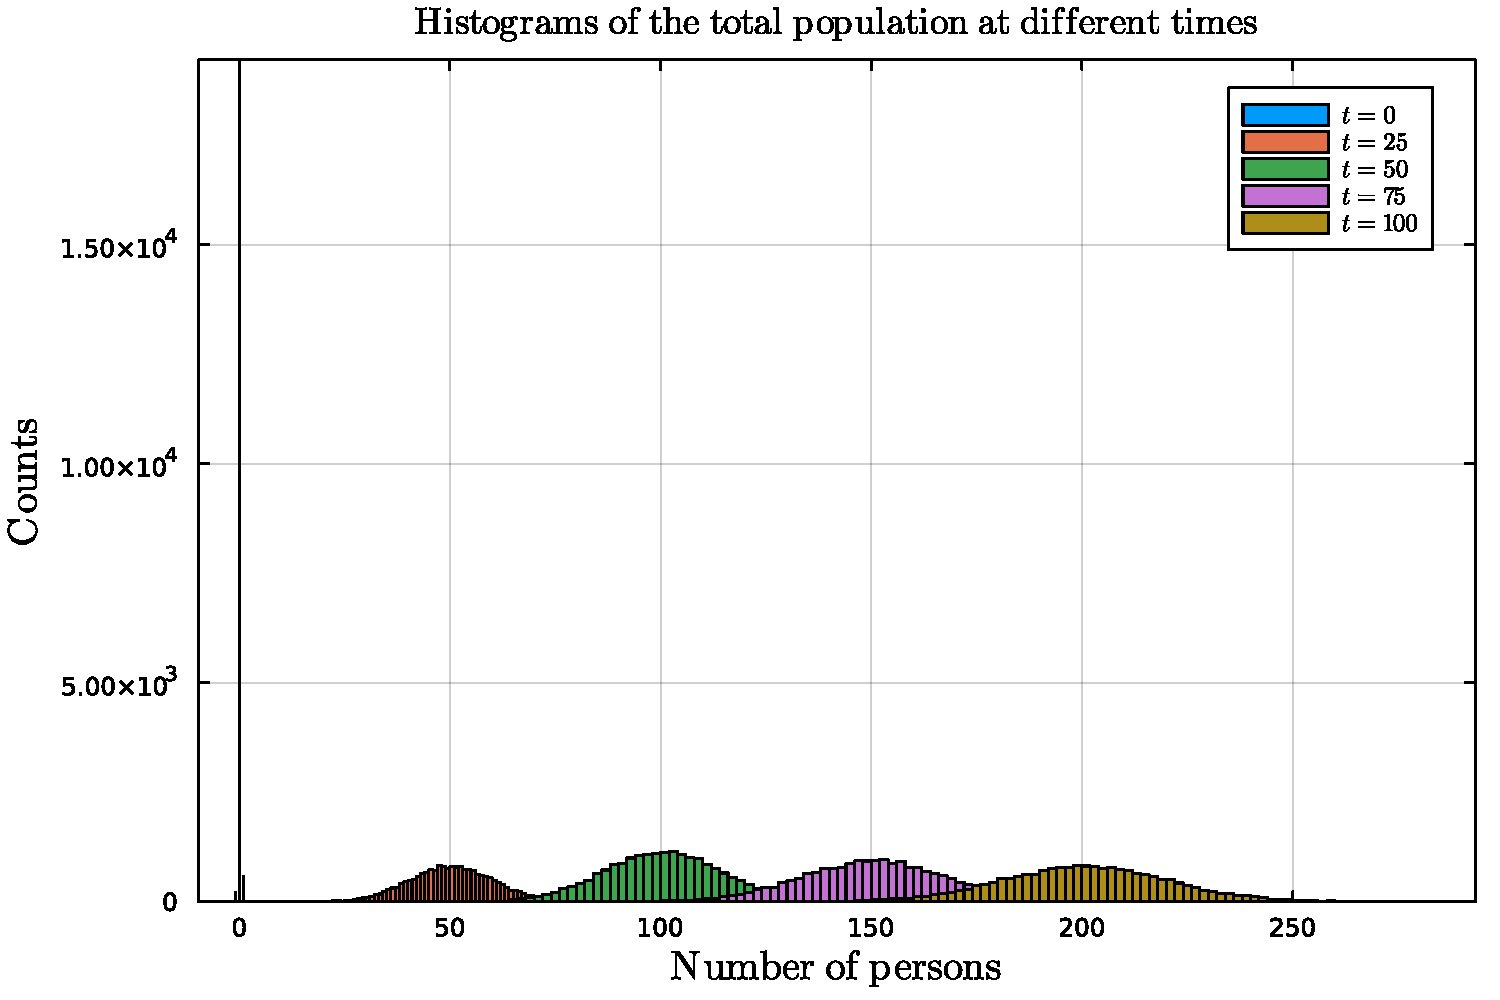
\includegraphics[width=0.8\textwidth]{imgs/hw5/bdProcessHistograms.pdf}
    \caption{Evolution of the number of persons modeled as a Poisson process with a data set of \num{20000} realizations in a time span of 100 days. }
    \label{fig:bdProcessHisto}
\end{figure}

As an interesting result, the same qualitative behavior of the distributions shown in figure \ref{fig:poissonProcessHisto} can be seen in figure \ref{fig:bdProcessHisto}, in which the mean of the distribution is shifting when the time passes and the distribution also spreads out at a increasing time.
Also both set of distributions reassembles to a binomial distribution and than can be explained with the central limit theorem, because we are adding up multiple random variables.
Moreover, the average and the variance with respect of time, figure \ref{fig:bdProcessMeanVar}, has the same linear relation as in figure \ref{fig:poissonProcessMeanVar}, with the differences of the slope.
In these case, the slope of the average is $\beta-\gamma$, meanwhile the slope of the variance is $\beta+\gamma$.

\begin{figure}[ht!]
    \centering
    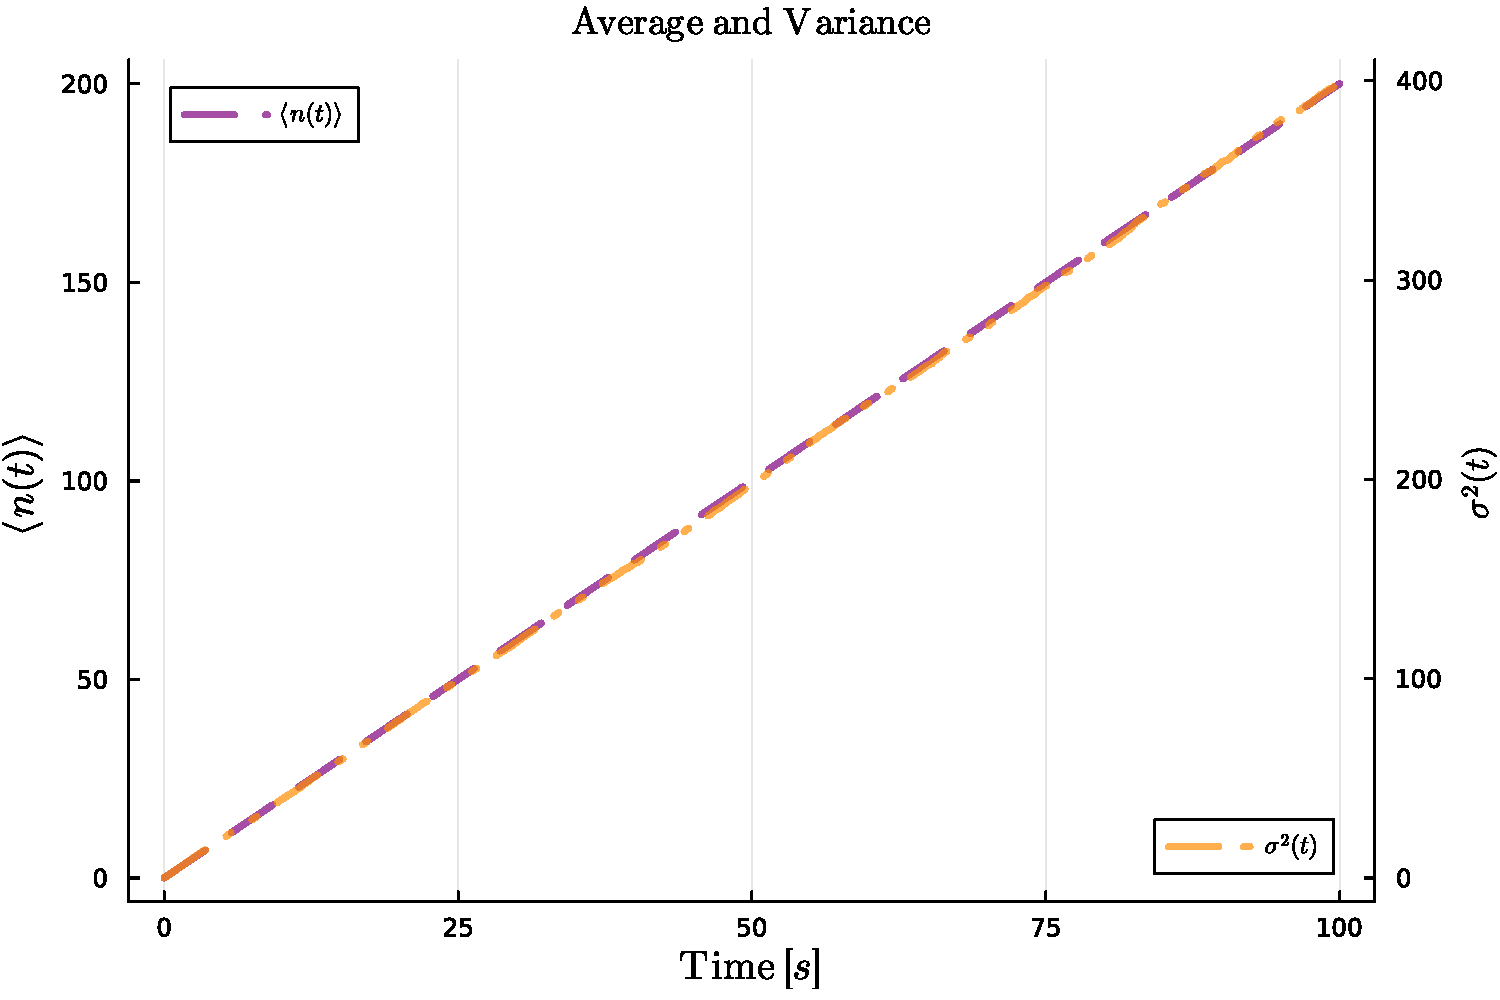
\includegraphics[width=0.8\textwidth]{imgs/hw5/bdProcessAvergeVariance.pdf}
    \caption{Mean and the variance of a data set of \num{20000} realizations of a  Poisson process in a time span of 100 seconds.}
    \label{fig:bdProcessMeanVar}
\end{figure}



% https://ocw.mit.edu/courses/18-440-probability-and-random-variables-spring-2014/60c8c00c94eebead998a50e9bb265b16_MIT18_440S14_Lecture13.pdf


\end{document}